\section{Introduction} \label{sec:intro}


\begin{table}
\begin{tabular*}{\columnwidth}{|l|p{0.76\columnwidth}|}
\hline
\bf Symbol		& \bf Meaning \\\hline
$QR_{q,R}$		& Range query from $q$ to all $o_i : d_{q,o_i} < R$) \\\hline
$\chi_{s,t}$		& The frequency of a \spath \\\hline
$P_{s,t}$		& A \spath from s to t \\\hline
$d_{s,t}$		& The \spath distance of a path $P_{s,t}$ \\\hline
$euclid_{s,t}$		& The euclidean distance of a path $P_{s,t}$ \\\hline
$\mathcal{O}$		& The set of $\poi \in \mathbf{V}$, the set of vertices\\\hline
$o_i$			& Element i in $\mathbf{O}$ \\\hline
$\mathcal{O}_{q,R}$	& The result set of  $Q_{q,R}$ \\\hline
$dist_O$ 		& Table of distances between vertices $v_s, v_t \in P_{s,t} :  P_{s,t} \in \spath_q$ \\\hline
$\spath_{q}$		& A set of \spath from q to all $o_i$ \\\hline

$\Psi$ 			& The Cache \\\hline
% $|SP|$			& Length of a \spath \\\hline
% $|\Psi|$		& Number of vertices in the cache \\\hline
% $\Phi(sp)$		& The set of all sub-paths in a \spath $sp$ \\\hline
% $\Phi^c(\Psi)$		& The set of all unique (sub-)paths in $\Psi$ \\\hline
% $\Gamma(\Psi)$		& Calculates the total utility of the content in the cache \\\hline 
$G\mathbf{(V,E)}$ 	& Graph representation of the Map \\\hline 
% $\mathbf{V}$ 		& The set of vertices in the Map \\\hline 
% WL			& Historical workload \\\hline
\end{tabular*}
\caption{Table of Symbols}
\label{tab:symbols}
\end{table}

\begin{algorithm}[bht]
\dontprintsemicolon
\SetVline

\SetKwInOut{Input}{input}\SetKwInOut{Output}{output}\SetKw{Return}{return}

\Input{

	$(q,R)$: A Range query\;
	$\mathcal{O}$: A set of POI \;
}

\Output{

	A set \poi $\in \mathcal{O}$ \;
}

 \funcc{Naive}{(q,R), \mathcal{O}}
{
    $tmpResult \leftarrow$ Check $\Psi$ for any $P_{q,o_i}$ \;
    \ForEach{$o_i \in \mathcal{O}$}
    {
      \If{$P_{q,o_i} \notin$ tmpResult}
      {	
	 $tmpResult \leftarrow$ Calculate $P_{q,o_i}$ \tcp{\emph{\spath from q to $o_i$}} \;
      }
    }

    \ForEach{$P_{q,o_i} \in$ tmpResult}
    {
      \If{$d_{q,o_i} < R$}
      {
	 $result \leftarrow P_{q,o_i}$ \;
      }
    }
    \Return{result} \;
}

\caption{Straightforward naive Algorithm}
\label{alg:naive}
\end{algorithm}


\begin{algorithm}[bht]
\dontprintsemicolon
\SetVline

\SetKwInOut{Input}{input}\SetKwInOut{Output}{output}\SetKw{Return}{return}

\Input{

	$(q,R)$: A Range query\;
	$\mathcal{O}$: A set of POI \;
}

\Output{

	A set \poi $\in \mathcal{O}$ \;
}

\funcc{Fair}{(q,R), \mathcal{O}}
{
    \ForEach{$o_i \in \mathcal{O}$ with euclidean distance < $R$ from $q$}
    {
      $pruned_{\mathcal{O}} \leftarrow o_i$ \;
    }
    result $\leftarrow$ \naivens((q,R), $pruned_{\mathcal{O}}$) \;

    \Return{result} \;
}

\caption{Fair Algorithm}
\label{alg:fair}
\end{algorithm}

\begin{algorithm}[bht]
\dontprintsemicolon
\SetVline

\SetKwInOut{Input}{input}\SetKwInOut{Output}{output}\SetKw{Return}{return}

\Input{
	A touple ($(q,R),\spath_q, dist_O$) \;
	$(q,R)$: Range query \;
	$\spath_{q}$: A set of \spath from q to all $o_i$ \;
	$dist_O$: table of distances between vertices\;
}

\Output{
	A set \poi $\in \mathcal{O}$ \;
}

\funcc{RSearch}{((q,R),\spath_q, dist_O)}
{
    using $\spath_q$ and $dist_O$ find all $P_{q,o_i}$ such that $d_{q,o_i}$ is smaller than R.\;

    \Return{$Q_{q,R}$} \;
}

\caption{Range search Algorithm}
\label{alg:rsearch}
\end{algorithm}

\begin{equation}
% QL: \{(q_0,R_0),\dots,(q_i,R_i)\}
% O: \{POI\}
\chi_{s,t}  = | P_{s,t} | \in ((q,R), \mathcal{O}) 
\end{equation}

\begin{definition}{ Range Search}\\
A range search query, denoted by $Q_{q,R}$ consist of a source vertice $q$ and a range $\mathbf{R}$.
The result of $Q_{q,R}$, denoted $\mathcal{O}_{q,R}$, is a set of objects $o_i \in \mathcal{O}$ with \spath distance $d_{s,t} \leq R$ on graph $G\mathbf{(V,E)}$.
\end{definition}


\begin{definition}{Range Search Query Log}\\
A range search query log $\mathcal{RQL}$ is a collection of timestamped queries that have been issued by users in the past.
A query is on the form $(q,R)$, where $q$ is a query point and $R$ is a range. The full form of the log, $\mathcal{RQL}$,  is then: $\{(q_0,R_0),\dots,(q_i,R_i)\}$
\end{definition}


Using a query log, $\mathcal{RQL}: \{(q_0,R_0),\dots,(q_i,R_i)\}$, we first need to expand each query into its \spath result set containing \spaths from $q$ to each \poi reachable within R distance on a roadnetwork. 
To find the result set of a query we use one of two algorithms: \naive or \fairns.

The \naive algorithm will not only find the result set of \spath for each query $\in QL$, but also the \spath from $q$ to all other possible \poins, before pruning and returning the result set of \poisns.
\naive does so by first finding all paths from $q$ to any \poi in the cache. Afterwards it will issue \spath queries from $q$ to the remaining \pois not already found via the cache. 
Once all paths are found \naive will prune the set of paths such that only the paths with distance < $R$ remain. This is the result so \naive returns it to the user.

The idea behind the \fair algorithm (see alg. \ref{alg:fair}) is to prune \poisns, which can not belong to the result set of a query, before doing range search. The \fair algorithm works by, for a query (q,R), first finding the set {\it tmp\poins}, of \pois which lay within euclidean distance $R$ of the query point $q$. \fair then invokes the \naive algorithm using {\it tmp\poins} as the set of \poins.






\begin{figure}[hbt]
  \center
        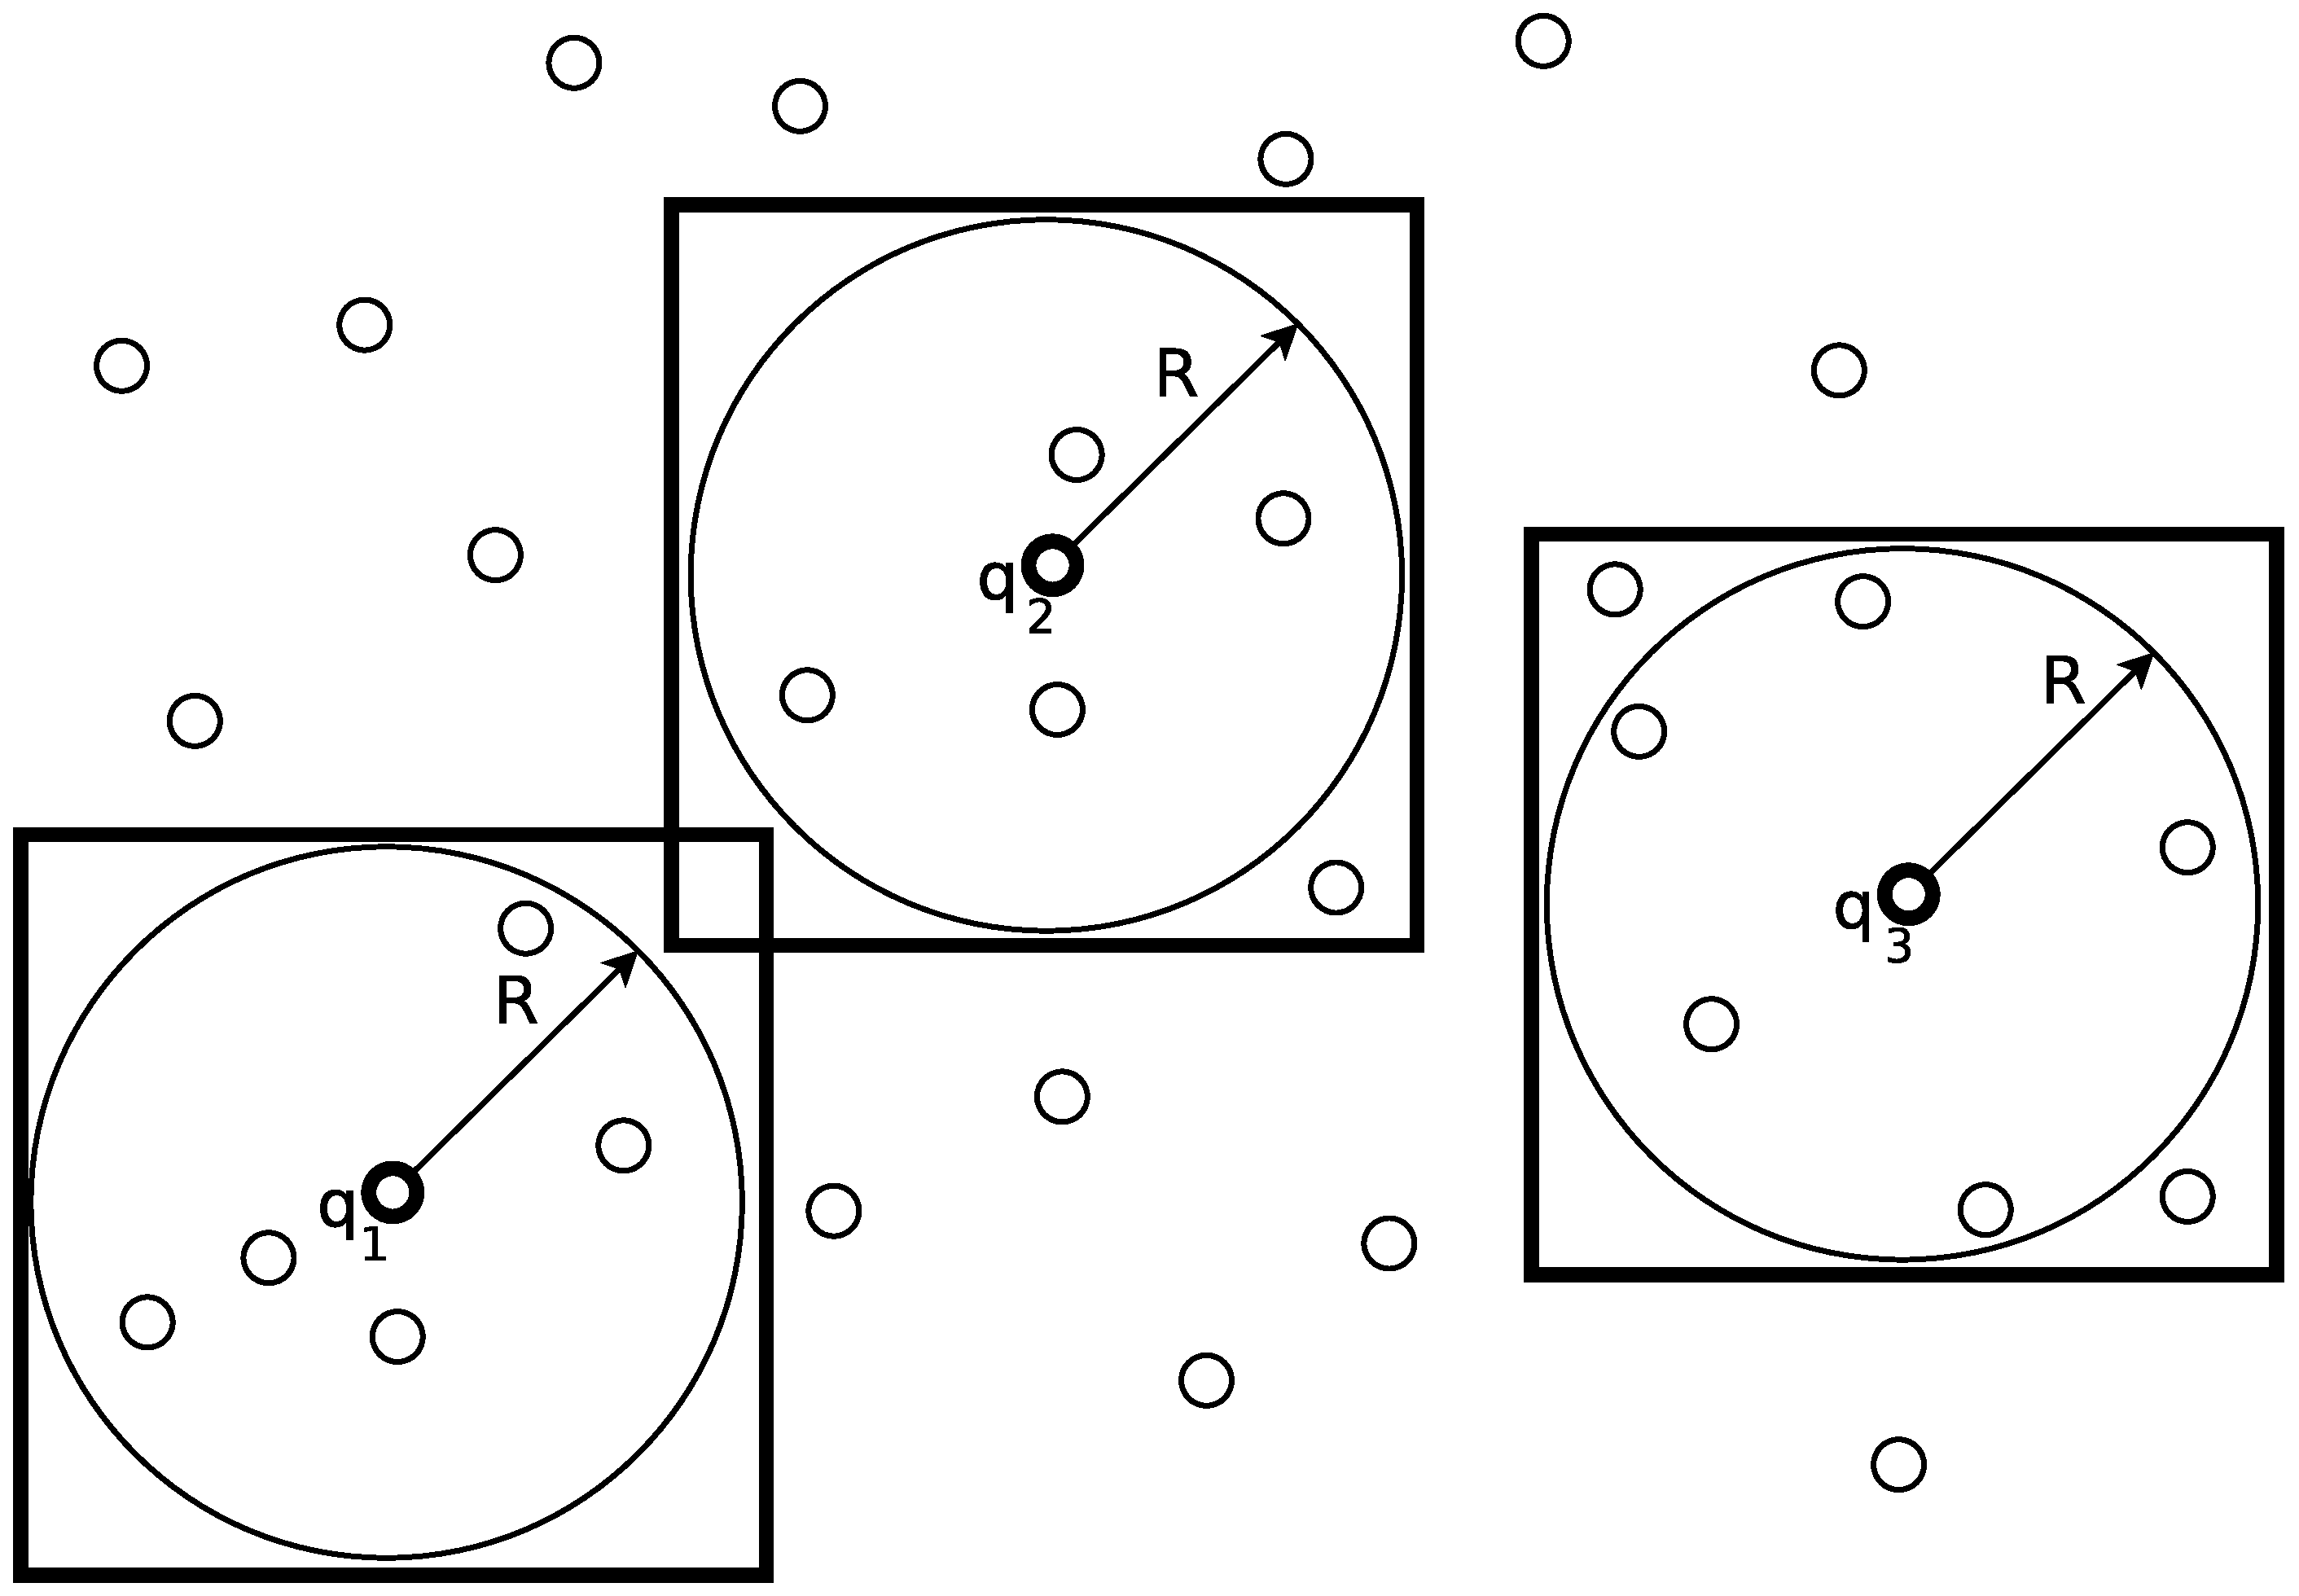
\includegraphics[width=0.45\textwidth]{figures/queryregions}
        \caption{Query points $q_1,q_2,q_3$, with region defined by R. White points are \poins}
  \label{fig:queryreg}
\end{figure}

\begin{figure}[hbt]
  \center
        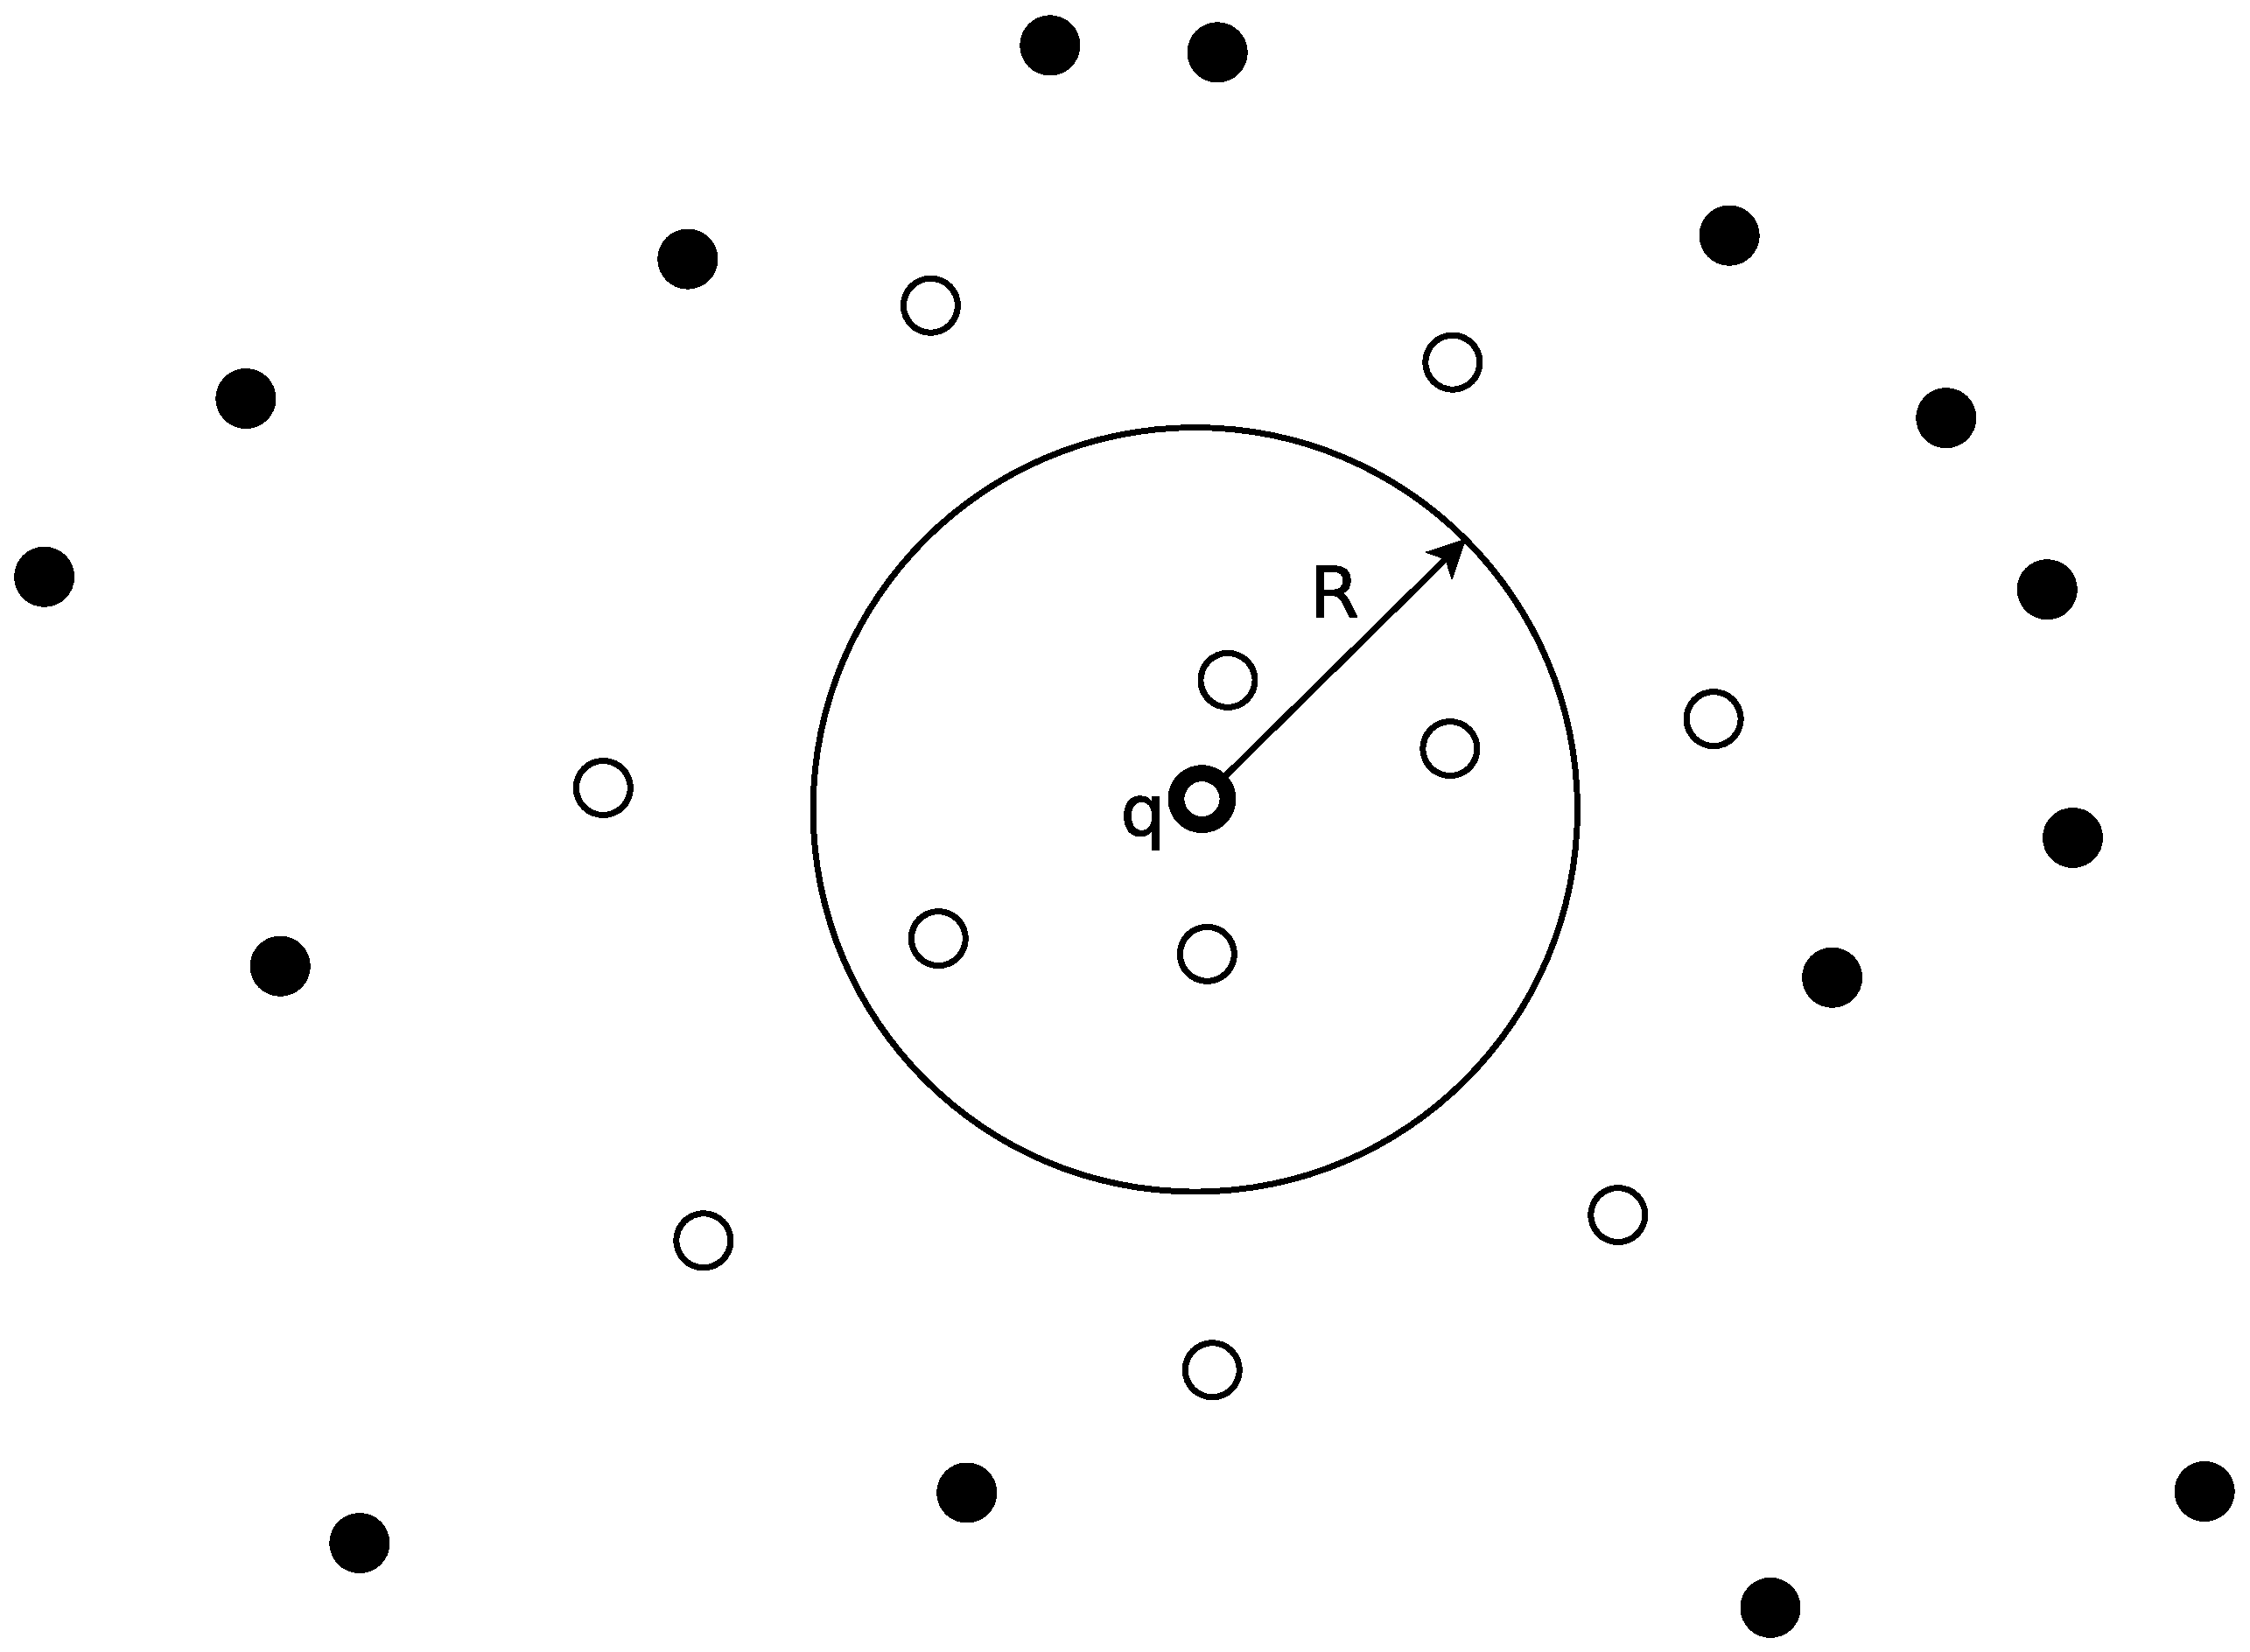
\includegraphics[width=0.45\textwidth]{figures/dominating}
        \caption{White points outside region R are dominating all black points}
  \label{fig:dominating}
\end{figure}